% !TeX spellcheck = en_GB 
\section{Conclusion}

interlocking can achieve 85\% of the strength of the PP and TPLA base materials; we reach about \todo{65\%}

diagonal design outperforms dovetail interlocking?

genus interlocking shows potential for high compliance materials

genus interlocking can help with complex and slanted surfaces 


\subsection{Applications}
explain: PP for living hinges; TPLA for stiffness


photo's of gripper, container, prosthetic hand 



\begin{figure}
	\centering
	\begin{subfigure}[B]{.33\columnwidth}
		\centering
		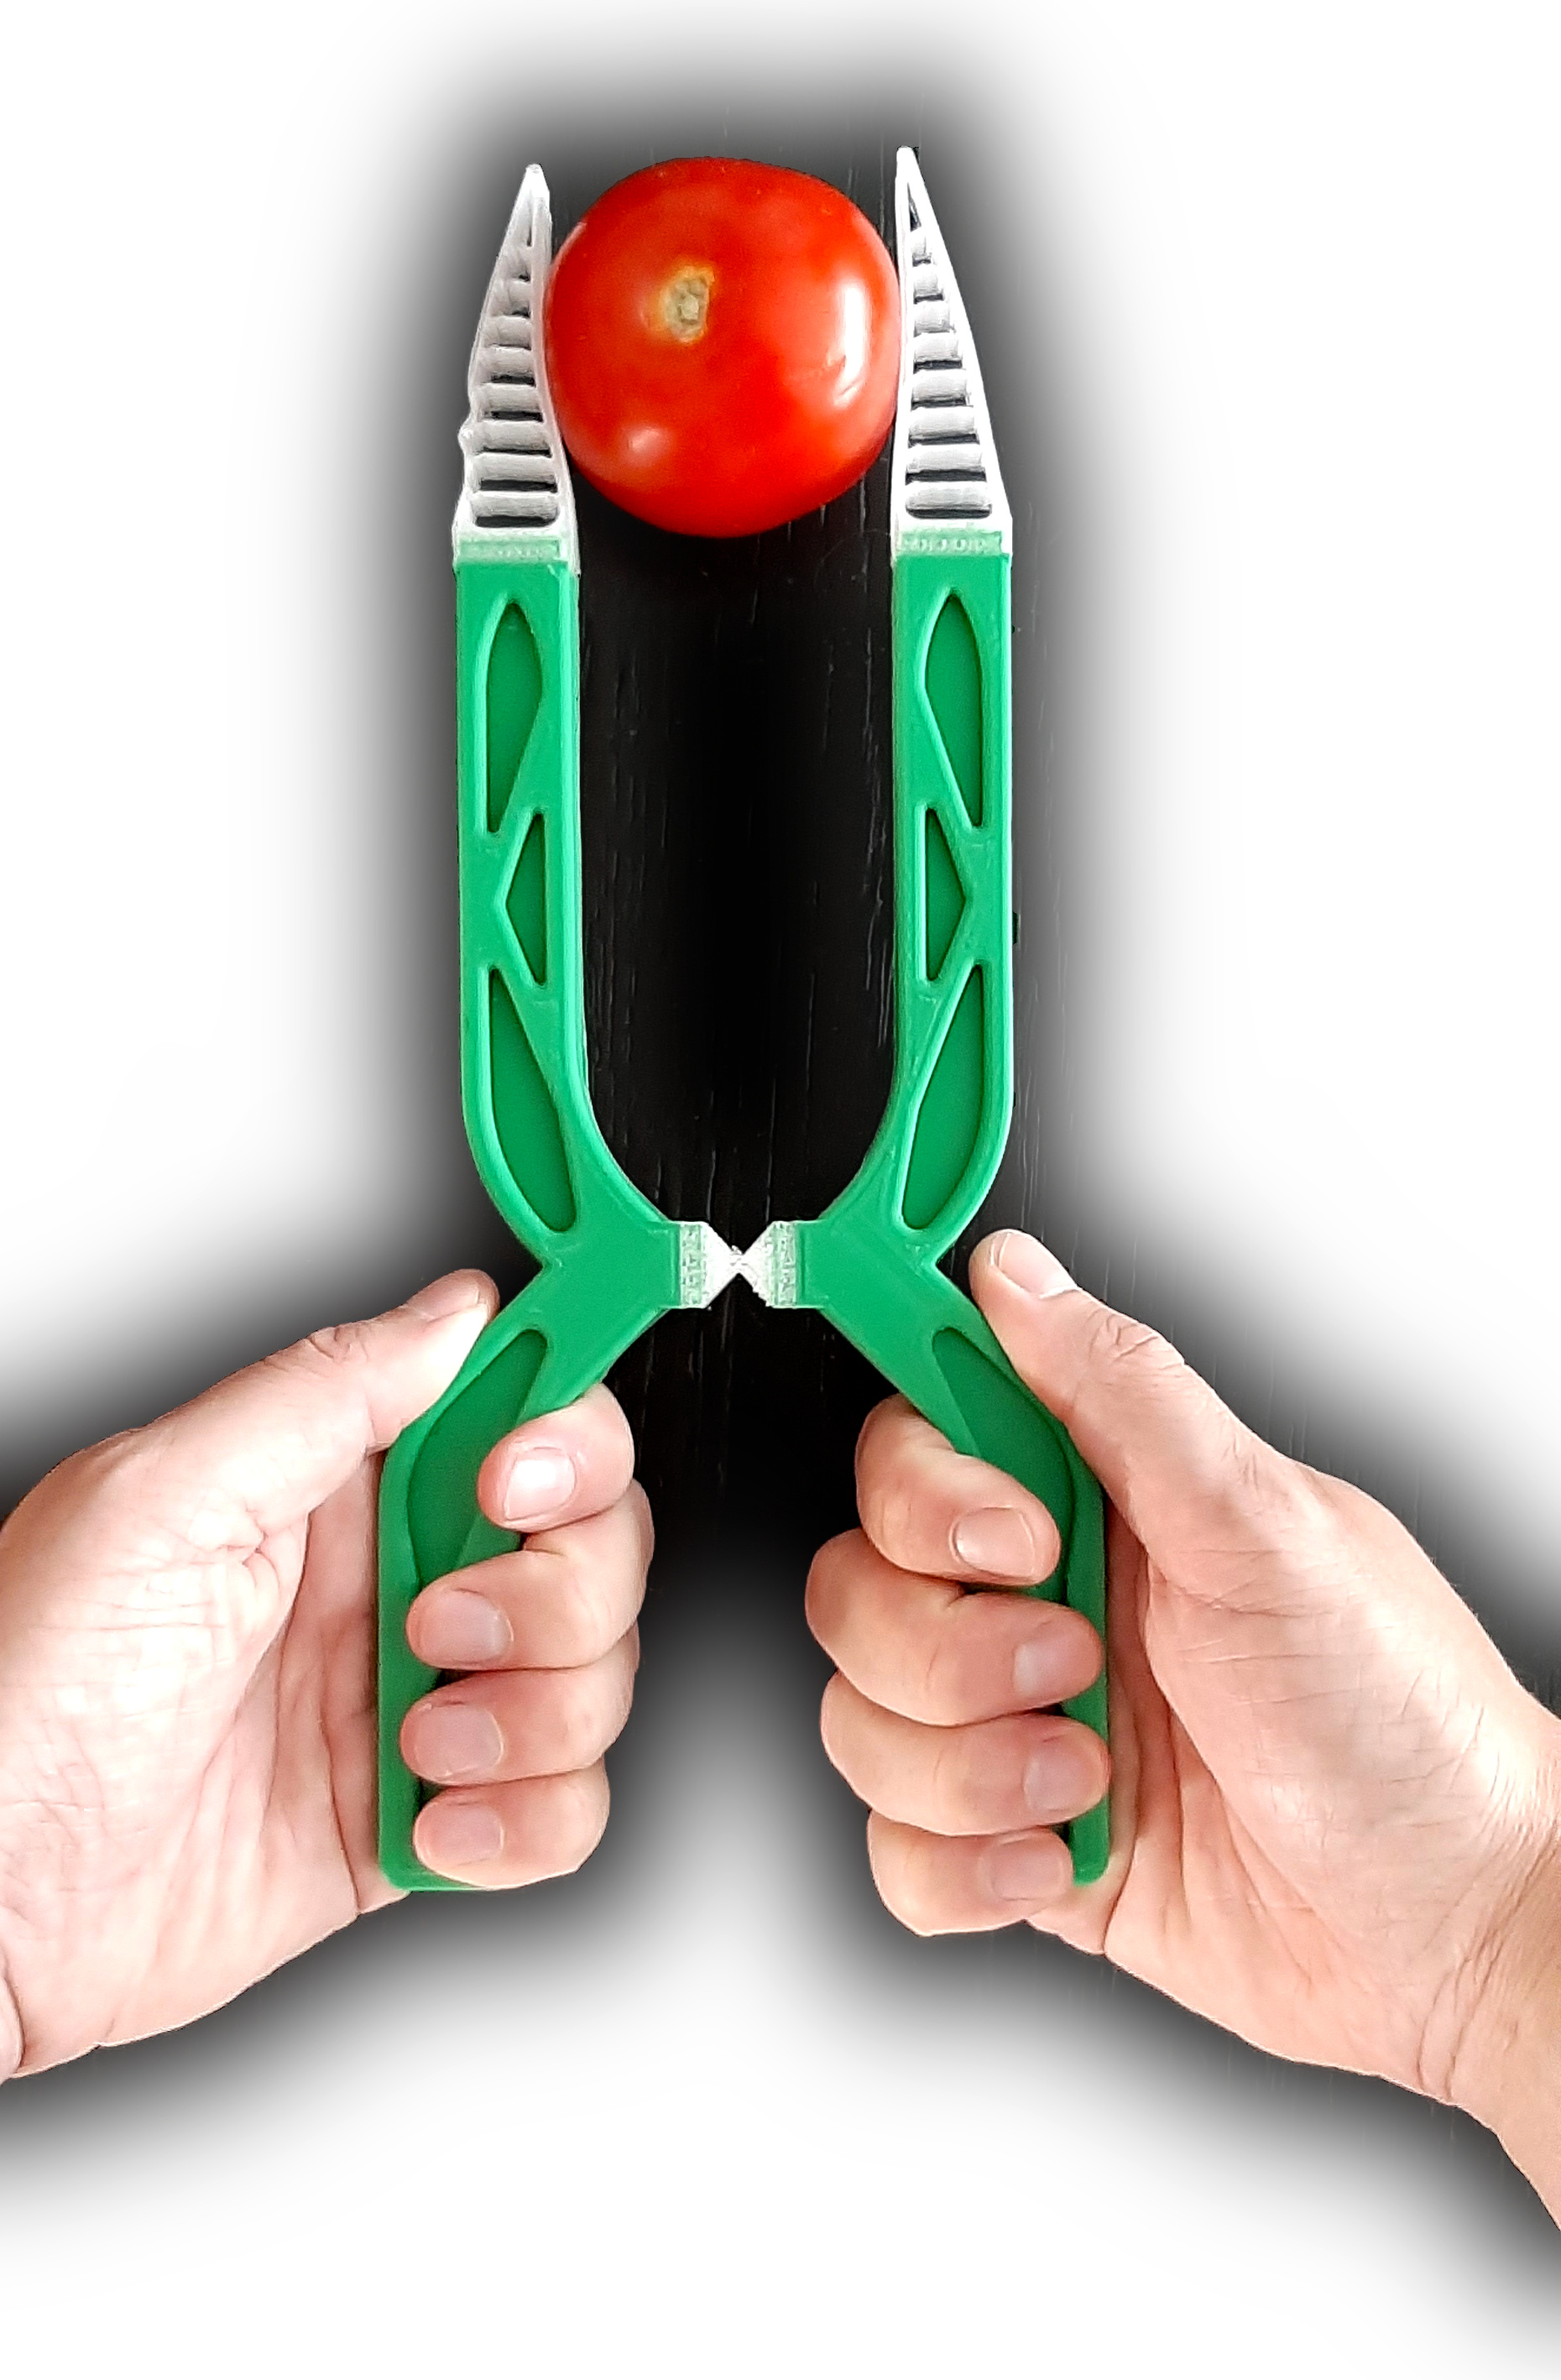
\includegraphics[width=\columnwidth]{sources/applications/gripper.jpg}
		\caption{Gripper design}
		\label{fig:gripper}
	\end{subfigure}
	\caption{Applications of interlocking structures.}
\end{figure}




\subsection{Future work}
Future work might be aimed at loading scenarios different from tensile, different materials, different nozzle sizes and different layer heights.
It is specifically compelling to investigate the resilience of the interlocking structure against vertically applied loads.
Another interesting route is to optimize for an interface between two bodies which has a complex geometry and heterogeneous stress distribution.

If the design constraint on the length of the transitional structure between the two material is released,
the manufacturing constraints are less relevant, which means that the geometry of the structure is less restricted.
The geometry of the microstructures could then be optimized for tailored mechanical properties.
In fact, such multi-material microstructures could be tailored for functionally graded materials.
With a relatively large geometry of the functionally graded multi-material lattice structure,
the IGIM lattice can again be used to ensure connectivity between the two materials,
while the meso-scale structure could be used to guarantee the functionally graded mechanical properties.
